\documentclass{beamer}
\usetheme{Madrid}

\usepackage{cmap}
\usepackage[T2A]{fontenc}
\usepackage[russian,english]{babel}
\usepackage[utf8]{inputenc}
\usepackage{amsmath, amssymb}
\usepackage{minted}
\usepackage{hologo}

\usepackage{algorithm2e}
\usepackage{algorithmic}
\usepackage{float}

\usepackage{cancel}
\usepackage{ulem}

% \newtcbox{\mybox}{blank, on line, opacitytext=0.5}

\title[Machine learning facilitation]{
	Preprocessing Sequential Data for Machine Learning Facilitation using Curriculum Learning
}

\author[Maxim Surkov]{
	{\footnotesize Project Proposal}\\
	Maxim K. Surkov, group BPM171\\
 	{\footnotesize Research Advisors: Ivan P. Yamshchikov}\\
 	{\footnotesize Linguistic Advisor: Department of Foreign Languages}
}
\institute[NRU HSE SPb]{
	Saint Petersburg School of Physics, Mathematics, and Computer Science\\
	Department of Computer Science
}
\date{6 april 2021}

\begin{document}

\frame{\titlepage}

\begin{frame}
\frametitle{Outline}
	\begin{itemize}
		\item Motivation and definitions
		\item Literature Review
		\item Methodology
		\item Results
	\end{itemize}
\end{frame}

\begin{frame}
	\frametitle{Motivation}
\begin{columns}
	\column{0.5\textwidth}
	\begin{itemize}
		\item social networks
		\item voice assistants
		\item translators
		\item chatbots
	\end{itemize}
	\column{0.5\textwidth}
	
\includegraphics[scale=0.2]{nlp_real_life.png}
\end{columns}
\noindent\makebox[\linewidth]{\rule{\paperwidth}{0.4pt}}
\begin{columns}
	\column{0.5\textwidth}
	\begin{itemize}
		\item classification
		\item machine translation
		\item natural language understanding
	\end{itemize}
	\column{0.5\textwidth}
	\begin{itemize}
		\item tiny language models
		\item GPT-3
			\begin{itemize}
				\item extremely large
			\end{itemize}
		\item {\bf BERT}
			\begin{itemize}
				\item high quality
			\end{itemize}
	\end{itemize}
\end{columns}
\end{frame}

\begin{frame}
	\frametitle{Motivation}
	\begin{itemize}
		\item pre-training
			\begin{itemize}
				\item required time: from 1-2 days to {\bf 1-2 weeks}
				\item world record: 47 minutes using {\bf 1472} GPUs

					\begin{table}
						\begin{tabular}{l|c}
							Dataset & Samples \\
							\hline\hline
							Wikipedia & 3-600M \\
							BooksCorpus & 74M\\
						\end{tabular}
					\end{table}
			\end{itemize}
		\item fine-tuning
			\begin{itemize}
				\item required time: 1-2 days

					\begin{table}
						\begin{tabular}{l|c}
							Dataset & Samples \\
							\hline\hline
							HND & 600k-2M \\
							s140 & 1.6M \\
							IWSLT & 200-230k \\
							QQP & 364k \\
							MNLI & 393k \\
						\end{tabular}
					\end{table}
			\end{itemize}
	\end{itemize}
\end{frame}

\begin{frame}
	\frametitle{Curriculum Learning. Definition}
	\begin{itemize}
		\item task: machine translation
		\item Models: BERT, LSTM
		\item Datasets: IWSLT'15, IWSLT'16, WMT'16
		\item Algorithm:
		\begin{columns}
			\column{0.5\textwidth}
			\begin{enumerate}
				\item sort samples by text complexity (length, log-likelihood)
				\item for $T$ steps (consider $t$-th step)
				\begin{itemize}
					\item calculate $c(t) \in [0, 1]$
					\item form the batch from $c(t)$ {\bf easiest} samples
					\item do training step
				\end{itemize}
			\end{enumerate}
			\column{0.5\textwidth}
			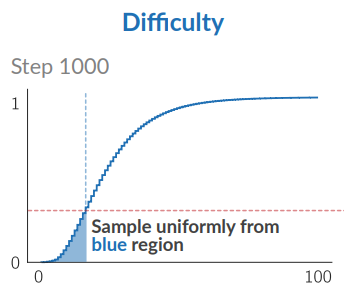
\includegraphics[scale=0.4]{acl19_algo.png}
		\end{columns}
	\end{itemize}
\end{frame}

\begin{frame}
	\frametitle{Research Field}
	\begin{table}
		\begin{tabular}{l|cccc}
			metric & classification & MT & pre-training & NLU \\
			\hline
			length & & $\checkmark$ & & \\
			{\it language features}\footnote[1]{van der Sluis et al. (2010) showed that there is poor correlation with real text complexity} & & & & \\
			entropy & & & & \\
			model-based & & & & $\checkmark$ \\
			word frequency based & & $\checkmark$ & & \\
			log-likelihood & & $\checkmark$ & & \\
			\hline
			? & & & & \\
			\hline
		\end{tabular}
	\end{table}
	\begin{itemize}
		\item length is the best metric now
		\item there is no universal approach
		\item classification and pre-training is not investigated
	\end{itemize}
\end{frame}

\begin{frame}
	\frametitle{Problem Statement}
	{\bf Goal:} speed up the BERT model’s training process at the
	expense of applying effective text complexity estimation metrics within the framework of
	curriculum learning on pre-training and classification tasks
	
	{\bf Problems:}
	\begin{enumerate}
		\item Suggest alternative text complexity metrics
		\item Implement a practical algorithm for metrics calculation on large datasets
		\item Carry out comparative analysis between the proposed metrics
		and the existing ones
		\item Study the impact of the found metrics on the BERT training
		time
	\end{enumerate}
\end{frame}

\begin{frame}
	\frametitle{Literature Review}
	\begin{table}
		\begin{tabular}{l|l}
			Bengio et al. (2009) & it was first shown that curriculum has a\\&great potential for improving ML models\\
			\hline
			Hacohen and Weinshall (2019)& application of curriculum learning in\\&computer vision\\
			Mermer et al. (2017) &\\
			\hline
			Platanios et al. (2019) & the first application of curriculum \\&learning in machine translation\\
			\hline
			Xu et al. (2020)& model-based metric investigation\\
			\hline
			Tom Kocmi et al. (2017) & good results on the machine translation\\&task were shown using curriculum learning\\&with {\bf length} and {\bf word frequency rank}\\&metrics\\
			Xuan Zhang et al. (2018)&\\
			\hline
			Nihat Ay et al. (2006) & Excess Entropy and TSE metrics\\& description \\
		\end{tabular}
	\end{table}
\end{frame}

\begin{frame}
	\frametitle{Methodology: metrics}
	\begin{itemize}
		\item filtered metrics
			\begin{itemize}
				\item length
				\item word frequency rank
				\item log-likelihood
				\item language metrics are {\bf not} used
			\end{itemize}
		\item Information Retrieval
			\begin{itemize}
				\item TF-IDF
			\end{itemize}
		\item Information Theory
			\begin{itemize}
				\item {\it Excess Entropy}
				\item {\it TSE}
			\end{itemize}
	\end{itemize}
\end{frame}

\begin{frame}
	\frametitle{Methodology: metrics calculation}
	\begin{itemize}
		\item Information Theory metrics adaption to texts
			\[
			T=(t_1, t_2, \ldots, t_{i-1},t_i,\ldots, t_n)
			\]
			\[
			t_i\rightarrow \xi^i_{t_i} =: \mu_i - \text{binary random value}
			\]
			\[
			\downarrow
			\]
			\[
			\xi=(\xi^1_{t_1},\xi^2_{t_2},\ldots,\xi^{i-1}_{t_{i-1}},\xi^i_{t_i},\ldots,\xi^n_{t_n})
			\]
		\item Statistics collection
			\begin{enumerate}
				\item divide the dataset into parts
				\item collect statistics on multiple processors in parallel
				\item join
			\end{enumerate}
		\item Excess Entropy and TSE metrics calculation
			\begin{enumerate}
				\item $\mathcal{O^*}(2^n)$
				\item $\mathcal{O}(n^2)$ - dynamic programming
				\item $\mathcal{O}(n)$ - math equations and text’s far-placed parts’ independence assumption
			\end{enumerate}
	\end{itemize}
\end{frame}

\begin{frame}
	\frametitle{Methodology: comparison method}
	\begin{enumerate}
		\item fix the dataset, model, and sampling algorithm
		\item train BERT model
		\item fix a sufficiently large accuracy value
			\begin{itemize}
				\item train BERT model without curriculum learning until convergence
				\item take the best accuracy value $\pm \varepsilon$
			\end{itemize}
		\item compare average number of steps required to reach this threshold
	\end{enumerate}
\end{frame}

\begin{frame}
	\frametitle{Results}
	\begin{table}
		\begin{tabular}{l|ccc|ccc}
			dataset & \multicolumn{3}{c}{HND (92.9\%)} & \multicolumn{3}{c}{s140 (85.5\%)}\\
			\hline
			sampler & CB & DB & Hyp & CB & DB & Hyp\\
			\hline
			length & 55k & 23k & 22.5k & 112.5k & 20k & 19k \\
			TF-IDF & $\infty$ & 19.5k & 24k & 115.5k & 21.5k & 19.5k \\
			TSE & 56.5k & 21k & 23k & 95.5k & 16.5k & 20.5k \\
			EE & 71.5k & 25.5k & 22.5k & 59k & 16.5k & 23k \\
			max wf rank & $\infty$ & 22k & 20.5k & 70k & 18.5k & 19.5k \\
			log-likelihood & $\infty$ & 20k & 24k & 112k & 17.5k & 21.5k\\
			\hline
			&&22k&&&18k&\\
		\end{tabular}
	\end{table}
\end{frame}

\begin{frame}
	\frametitle{References}
	
\end{frame}

\end{document}